\section{Thiết kế phương pháp và lý do lựa chọn}
\label{sec:method}
\subsection{Luồng xử lý và trạng thái triển khai}
Hình~\ref{fig:pipeline} phân biệt các nhánh đã hiện thực hóa với nhánh dự kiến.
Dữ liệu raw là đầu vào bất biến. Reader và validator tạo quan sát cùng nhãn RUL
train trong bộ nhớ; EDA và suy luận M2.3a chỉ dùng train, đồng thời đã xuất
bảng, hình hoặc metadata tương ứng. M3.1 đã ghi observations và train targets
vào Silver Parquet, đồng thời tạo Gold engine summary ở Parquet và SQLite.
M3.2 đã tạo Gold rolling features từ Silver observations.

\begin{figure}[H]
\centering
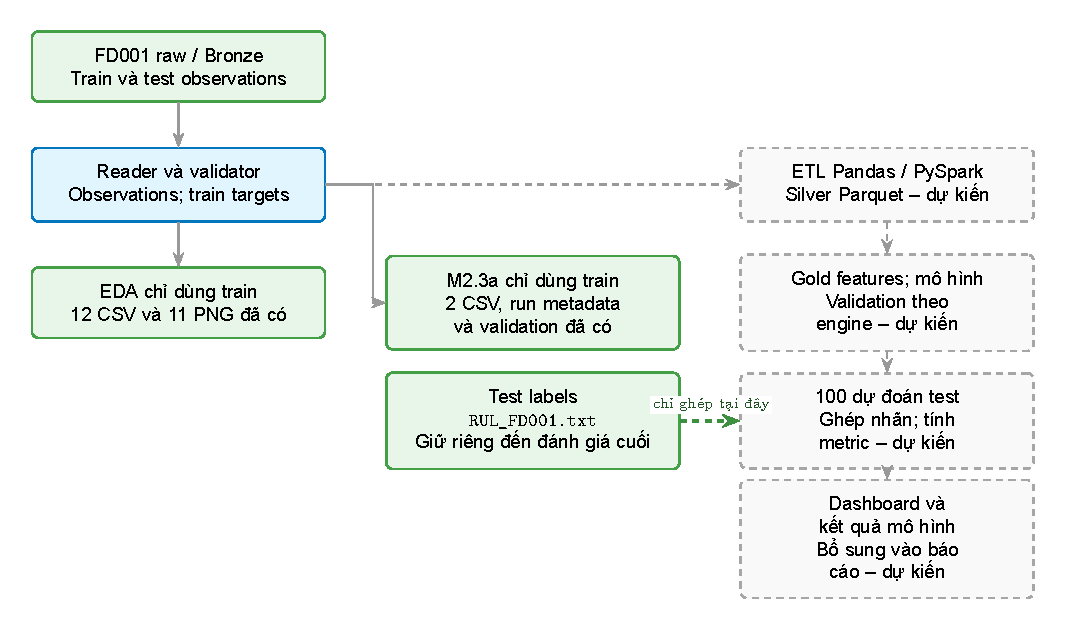
\includegraphics[width=0.98\linewidth]{figures/pipeline.pdf}
\caption[Luồng dữ liệu và trạng thái triển khai]{Luồng dữ liệu: đường liền thể
hiện nhánh đã hiện thực hóa hoặc đã có artifact; đường và khung nét đứt thể hiện
phần dự kiến. Nhãn test được vẽ như side input tách riêng và chỉ ghép vào bước
đánh giá cuối.}
\label{fig:pipeline}
\end{figure}

Bronze giữ dữ liệu nguồn để truy vết. Silver lưu observations đã gán kiểu dữ
liệu và train targets trong Parquet; Gold M3.1 lưu engine summary trong
Parquet/SQLite để kiểm tra boundary và truy vấn cục bộ. Gold M3.2 lưu rolling
features trong Parquet, tách khỏi bước fit scaler hoặc mô hình. Cách tách lớp
giúp phân biệt dữ liệu gốc với dữ liệu suy ra và xác định bước gây mất hoặc
nhân bản dòng.
Pandas là reference implementation; PySpark tái hiện ba boundary và parity
checker đã xác nhận ba bảng khớp với sai khác lớn nhất bằng 0 trong lần chạy
local có JRE. Chưa có bằng chứng để kết luận công cụ nào nhanh hơn.

FD001 có dung lượng nhỏ. Benchmark M3.1 ở mức $1\times$, $10\times$ và
$100\times$ chỉ đánh giá chi phí tạo engine summary; bản nhân dữ liệu đổi engine
ID và tách khỏi phân tích khoa học. Việc nhân bản quan sát không tạo thêm động
cơ độc lập để huấn luyện hoặc thu hẹp khoảng tin cậy.

\subsection{EDA theo đơn vị động cơ}
EDA chỉ sử dụng train để tìm hiểu dữ liệu mà không dựa vào test khi quyết định
phương pháp. Phân phối tuổi thọ tính mỗi động cơ một lần. Ngược lại, histogram
RUL theo quan sát cho động cơ sống lâu nhiều quan sát hơn. Hai cách tổng hợp trả
lời hai câu hỏi khác nhau và không được diễn giải thay thế nhau.

Correlation giữa sensor và RUL được tính bằng Spearman riêng trong từng động
cơ, sau đó tóm tắt phân phối giữa các động cơ. Lựa chọn này khảo sát liên hệ đơn
điệu và tránh để số dòng của một động cơ quyết định trực tiếp trọng số trong
bảng tổng hợp correlation. Tuy vậy, dependence theo thời gian vẫn tồn tại;
correlation mô tả chưa chứng minh quan hệ nhân quả hoặc hiệu quả dự đoán ngoài
mẫu.

Sensor hằng có correlation không xác định, được giữ dưới dạng NaN thay vì gán
0. Ba động cơ minh họa được chọn gần các tứ phân vị tuổi thọ; nếu bằng khoảng
cách, chọn ID nhỏ hơn. Quy tắc này dựa trên tuổi thọ, không dựa trên quỹ đạo
sensor có hình dạng dễ quan sát. Quỹ đạo hiện có biểu diễn giá trị gốc theo
cycle, không smooth; mỗi ô dùng thang đo riêng. Ba động cơ này không đại diện
thống kê. Tuổi thọ đầy đủ chỉ dùng cho phân tích hồi cứu sau khi đã quan sát cả
chuỗi, không được dùng làm feature dự đoán tại cycle hiện tại.


\subsection{Đặc trưng từ window M3.2}
Biểu diễn chính đã triển khai là trailing window (cửa sổ chỉ chứa hiện tại và
quá khứ) dài 30 cycles. Ví dụ, dự đoán tại cycle 170 dùng các cycle 141--170
của cùng động cơ. Mỗi output row khóa bởi \texttt{(split, engine\_id, cycle)},
trong đó \texttt{cycle} là cycle cuối của window. Transformer từ chối engine có
ít hơn 30 cycles; không padding, không impute và không rút ngắn window.

M3.2 giữ đủ 21 sensors trong artifact để chưa thực hiện feature selection trên
toàn bộ train. Với mỗi sensor, pipeline tạo sáu đặc trưng theo mẫu
\texttt{<sensor>\_\_<stat>}: giá trị cuối, mean, sample standard deviation
(\texttt{ddof=1}), min, max và linear slope theo vị trí 1--30 trong window. Nếu
một sensor bằng đúng số cycle trong window 1--30 thì các feature tương ứng là
\texttt{last=30}, \texttt{mean=15,5}, \texttt{min=1}, \texttt{max=30} và
\texttt{slope=1}. Sample standard deviation dùng quy ước thống kê mẫu để nhất
quán với cách mô tả biến thiên trong EDA, nhưng quyết định này được ghi riêng
trong \filepath{outputs/features/run\_info.json} thay vì suy ngầm từ default.

Artifact hiện có 27.927 rows, gồm 17.731 train windows và 10.196 test windows.
Bước này không đọc \filepath{data/raw/RUL\_FD001.txt}, không join nhãn test,
không fit scaler, không chọn sensor và không huấn luyện mô hình. Các lựa chọn
phụ thuộc dữ liệu như loại sensor hằng, PCA hoặc scaler vẫn phải học trong
training fold ở mốc mô hình.

\subsection{Mô hình và đánh giá: phần dự kiến}
Naive baseline theo trung vị RUL cung cấp mốc so sánh khi không dùng tín hiệu
sensor. Ridge là baseline tuyến tính có regularization; HistGradientBoostingRegressor
là ứng viên phi tuyến. So sánh này nhằm đánh giá lợi ích của tín hiệu sensor so
với dự đoán đơn giản và mức cải thiện khi cho phép quan hệ phi tuyến. Chưa có
hyperparameter search hoặc kết quả để xếp hạng ba phương pháp.

Model selection dự kiến dùng GroupKFold 5-fold theo \texttt{engine\_id}. Các
window liền nhau của một động cơ có thể dùng chung phần lớn quan sát: hai window
141--170 và 142--171 dùng chung 29 cycles. Nếu chia ngẫu nhiên theo dòng, những
window gần như giống nhau có thể nằm ở cả train và validation, gây data leakage
(rò rỉ dữ liệu). Vì vậy, toàn bộ window của một động cơ phải thuộc cùng fold;
scaler, lựa chọn sensor và mô hình chỉ fit trên training fold.

Metric chọn mô hình dự kiến là mean engine-level MAE. Với $m$ động cơ validation
và $n_i$ dự đoán được đánh giá của động cơ $i$, đặt
\begin{equation}
\mathrm{MAE}_{\mathrm{engine}}=\frac{1}{m}\sum_{i=1}^{m}\left[\frac{1}{n_i}\sum_{t\in\mathcal E_i}|y_{i,t}-\widehat y_{i,t}|\right],
\end{equation}
trong đó $\mathcal E_i$ là tập cycle được protocol chọn để đánh giá. Cách lấy
trung bình này cho mỗi động cơ trọng số bằng nhau. Quy tắc chọn $\mathcal E_i$
trong cross-validation còn phải được cụ thể hóa và lưu cùng cấu hình trước khi
huấn luyện. RMSE và NASA asymmetric score dự kiến là metric phụ; chưa có số liệu
cho các metric này.

Sau khi chọn cấu hình bằng train/validation, mô hình được refit trên toàn train
và tạo một dự đoán cho mỗi động cơ test tại cycle cuối quan sát. Chỉ sau đó mới
ghép nhãn test để đánh giá cuối. Khoảng tin cậy dự kiến dùng bootstrap theo động
cơ nhằm giữ nguyên đơn vị chuỗi, thay vì giả định các window chồng lấn là mẫu độc
lập.

\subsection{Thống kê hiện có và ARIMA dự kiến}
M2.3a--M2.3b so sánh trung bình 30 cycles đầu và 30 cycles cuối trong cùng động cơ,
theo quyết định ngày 22/09/2026. Helper tạo cặp và các hàm suy luận theo sensor
đã được hiện thực hóa, kiểm tra bằng fixture và chỉ xử lý train. Notebook 02 đã
xuất bảng cặp, bảng suy luận, metadata, validation và hai hình panel tại
\filepath{outputs/statistics/}; bảng cặp có 2.100 dòng và bảng suy luận có 21
dòng. Mục~\ref{sec:stat-protocol} định nghĩa cặp, chiều chênh lệch, đầu ra,
giả định và cấu hình M2.0 đã chốt. Mục~\ref{sec:theory} trình bày cơ sở của
chênh lệch cặp trung bình, khoảng tin cậy bootstrap 95\%, Wilcoxon và
Benjamini--Hochberg FDR. Hình phân phối và effect size được tạo theo panel
riêng cho từng sensor, kèm diễn giải về sensor hằng, dấu chênh lệch và
heterogeneity giữa các engine. Kết quả M2.3a--M2.3b không phải feature
selection và không kết luận về hiệu quả dự đoán RUL.

ARIMA là phân tích phụ trên Health Index từ PCA được fit trong training fold.
ARIMA không áp dụng trực tiếp lên nhãn RUL train vì Công thức~\ref{eq:rul} tạo
một countdown tất định; dự báo lại countdown không chứng minh khả năng khai thác
tín hiệu sensor. Kế hoạch hiện tại chọn 10 động cơ validation đại diện, dùng
70\% đầu chuỗi để fit và 30\% cuối để đánh giá. Cách chọn động cơ cụ thể và
ARIMA order còn chưa triển khai. Kết quả sẽ cần ADF, Ljung--Box, forecast
MAE/RMSE và coverage của khoảng dự đoán 95\%.
